\documentclass{beamer}
\usepackage{tikz}
\usepackage{geometry}
\usepackage{graphicx}
\usepackage{siunitx}
\usepackage{amsmath}
\usepackage{amssymb}
\usepackage{amsbsy}
\usepackage{enumerate}
\usepackage{multirow}
\usepackage{indentfirst}
\usepackage{float}
\usepackage{mathrsfs}
\usepackage{xcolor}
\usepackage{hyperref}
\newcommand{\e}[1]{\times10^{#1}}
\newcommand{\degree}{^\circ}
\newcommand{\spl}[1]{\[\begin{split}{#1}\end{split}\]}
\newcommand{\enum}[1]{\begin{enumerate}{#1}\end{enumerate}}
\newcommand{\dd}{\text{d}}
\newcommand{\LA}{\Leftarrow}
\newcommand{\RA}{\Rightarrow} 
\newcommand{\LR}{\Leftrightarrow}
\newcommand{\m}{\backslash}
\newcommand{\ggp}[1]{\left<{#1}\right>} 
\newcommand{\outline}{\begin{frame}{Outline}\tableofcontents[currentsubsection]\end{frame}}
\newcommand{\mypause}{\ifpre\pause\fi}
\newcommand{\n}{\mathbb{N}_{def}}
\newcommand{\p}[1]{\mathscr{P}({#1})}
\newcommand{\pow}[2]{\mathscr{P}_{#1}({#2})}
\hypersetup{urlcolor=blue}
\usetheme{CambridgeUS}
\usecolortheme{dolphin}

\tikzstyle{every node}=[circle, draw, fill=blue!50,
inner sep=0pt, minimum width=4pt]

\setbeamertemplate{sidebar right}
{
  \vfill%
  \llap{\insertlogo\hskip0.1cm}%
  \vskip2pt%
  %\llap{\href{http://tex.stackexchange.com/}{See github: Paraphrase to Zach's "Easy" Derivation}\hskip0.2cm}% NEW
  \vskip3pt% NEW
  \llap{\usebeamertemplate***{navigation symbols}\hskip0.1cm}%
  \vskip2pt
}

\newif\ifpre
\pretrue

\begin{document}

\title{VE203 Review Class Week 7}
\institute[FA2018 VE203]{}
\author{Tianyi Ge}
\date{Fall 2018}
\maketitle

\section{RC Week 7}
\subsection{Induction}
\outline

\begin{frame}{Pure Set Theory}
    \begin{itemize}
        \item The only objects are sets
        \item Like $\{\emptyset\}$, $\{\{\emptyset\},\emptyset\}$, etc.
    \end{itemize}
    \begin{definition}
        Let $V$ be the set of all sets. $L$ is the set of all sets that have $\emptyset$ as a member. $$L=\{x\in V|\emptyset\in X\}$$
    \end{definition}
    \begin{itemize}
        \item $(L,\subseteq)$ is a complete lattice because every subset $A\subseteq L$ has both l.u.b. ($\bigvee A$) and g.l.b ($\bigwedge A$).
    \end{itemize}
\end{frame}

\begin{frame}{Successor Operation}
    \begin{definition}
        $S: V\to V$, $$S(x)=x\cup\{x\},\quad\forall x\in V$$
    \end{definition}
    \begin{definition}
        $F: L\to L$, $$F(A)=A\cup S"A, \quad\forall A\in L$$
    \end{definition}
    \begin{itemize}
        \item Successor operation operates sets (object-level).
        \item $F$ treats $A$ the set of sets (set-level).
        \item E.g. $S(\emptyset)=\emptyset\cup\{\emptyset\}=\{\emptyset\}$
        \item E.g. $F(\{\emptyset\}) = \{\emptyset\}\cup \{S(\emptyset)\}=\{\emptyset, \{\emptyset\}\}$
    \end{itemize}
\end{frame}

\begin{frame}{A flawed definition of $\mathbb{N}$}
    \begin{itemize}
        \item Further, $F$ is order-preserving.
        \item According to \emph{Tarski-Knaster Theorem}, $F$ has at least a fixed point, i.e. $F(X)=X\cup S"X = X$.
        \item In other words, if you take arbitrary element $x$ in $X$ and do successor operation once, you will find that the result $S(x)$ is still in $X$.
        \item We define the $\subseteq-$least fixed point as $\mathbb{N}_{def}$.
    \end{itemize}
    \spl{
        0&:=\emptyset\\
        1&:=S(\emptyset)=\{\emptyset\}\\
        2&:=S(S(\emptyset)) = \{\emptyset, \{\emptyset\}\}\\
        \vdots
    }
\end{frame}

\begin{frame}{A flawed definition of $\mathbb{N}$}
    \begin{example}
            $$\{0,1,2\} \LR \boldsymbol{\{\emptyset,\{\emptyset\}, \{\emptyset,\{\emptyset\}\}\}}$$
            $$F(\{0,1,2\})=\{0,1,2,3\}$$
    \end{example}
    \begin{itemize}
        \item To get 3, we treat the current set $\{0,1,2\}$ as the new element and put it into our new set.
    \end{itemize}
    \spl{
        3\LR&\quad\boldsymbol{\{\emptyset,\{\emptyset\}, \{\emptyset,\{\emptyset\}\}\}}\\
        &\quad\Downarrow\\
        \{0,1,2,\boldsymbol{3}\} \LR \{\emptyset,\{\emptyset\}, \{\emptyset,\{\emptyset\}\}, &\quad\boldsymbol{\{\emptyset,\{\emptyset\}, \{\emptyset,\{\emptyset\}\}\}}\quad\}
    }
    \begin{itemize}
        \item The natural number matches the cardinality of the corresponding set
    \end{itemize}
\end{frame}

\begin{frame}{A flawed definition of $\mathbb{N}$}
    \begin{itemize}
        \item Now we know that $F(\mathbb{N}_{def})=\mathbb{N}_{def}$
        \item $\mathbb{N}_{def}$ is the $\subseteq$-least fixed point, which means any other fixed point $X$ ($\emptyset \in X$) satisfies that $\mathbb{N}_{def}\subseteq X$.
    \end{itemize}
    \begin{theorem}
        The order $\leq$ is a well ordering of $\mathbb{N}_{def}$.
    \end{theorem}
    
    \begin{theorem}
        $\mathbb{N}_{def}$ satisfies the principle of induction: If a property $P(x)$ is such that $P(0)$ holds, and for all n ∈ N def, if $P(n)$ holds, then $P(n+1)$ holds, then for all $n \in\mathbb{N}_{def}$, $P(n)$ holds
    \end{theorem}

\end{frame}

\begin{frame}{Principle of Induction in $\n$}
    \begin{itemize}
        \item If principle of induction does not hold, then for some $n\in\n$ $P(n)$ does not hold.
    \end{itemize}
    \begin{proof}
        Let $A=\{n\in\n|P(n)\}\subset \n$, also $\emptyset\in A$. Thus $A$ becomes the least fixed point rather than $\n$. 
    \end{proof}
\end{frame}

\begin{frame}{Steps for Induction}
    \begin{block}{Steps}
    \begin{enumerate}
        \item Define the property $P(n)$ properly.
        \item Show that $P(n_0)$ holds. $n_0$ is not necessarily $0$.
        \item Show that $\forall n\in\mathbb{N}$ with $n\geq n_0$, $P(n)\RA P(n+1)$. Use the result from $P(n)$ to derive $P(n+1)$.
        \item Conclusion.
    \end{enumerate}
    \end{block}
\end{frame}

\begin{frame}{Strong Induction}
    \begin{block}{Steps}
        \begin{enumerate}
            \item Define $A(n)$ properly.
            \item Show that $A(n_0)$ holds.
            \item Show that $\forall n\geq n_0$, if for all $n_0\leq k\leq n$, $A(k)$ holds, then $A(n+1)$ holds.
            \item Conclusion.
        \end{enumerate}
    \end{block}
    \begin{itemize}
        \item Strong induction allows using all the proved previous conclusions to derive the next, rather than only the previous one.
    \end{itemize}
\end{frame}

\begin{frame}{Recursive Defined Functions}
    \begin{enumerate}
        \item $f(0)=n_0$ (initial condition).
        \item $G(n,f(n))=(n+1,f(n+1))$ (rule).
        \item $X=\{R\in \mathcal{P}(\mathbb{N}\times\mathbb{N})|(0,n_0)\in R\}$
        \item $X$ is a complete lattice because arbitrary set $A\subseteq X$ satisfies that $\bigwedge A=\bigcap A$ and $\bigvee A=\bigcup A$ ($(0,n_0)\in\bigcap A$).
        \item $F:X\to X$ with $F(R)=R\cup G"R$ is order preserving ($R\subseteq T\Rightarrow F(R)\subseteq F(T)$).
        \item There exists a least $f$ in $X$ s.t. $F(f)=f\cup G"f=f$ (why least?).
        \item Thus $f$ represents $\{(0,f(0)), (1,f(1)),\hdots\}$.
    \end{enumerate}
\end{frame}

\begin{frame}{Structural Induction}
    \begin{definition}
        \begin{itemize}
            \item A is $\subseteq$-least, $B\subseteq A$, $A$ is closed under $C_1,\cdots,C_n$.
            \item For all $b\in B$, P(b) holds
            \item For all $a_1,\cdots,a_m$ and $c$ and $1\leq i\leq n$, if $P(a_1),\cdots,P(a_m)$ all hold and $c$ is obtained from $a_1,\cdots,a_m$ by a single application of $C_i$, then $P(c)$ holds
        \end{itemize}
    \end{definition}
    \begin{itemize}
        \item Use part of the proved conclusions to derive the next one. The index of next conclusion is determined by some defined principle $C_i$.
    \end{itemize}
\end{frame}

\subsection{Counting}
\outline
\begin{frame}{Subsets of size $k$}
    \begin{definition}
        Let $A$ be a finite set and $0\leq k\leq |A|$, then $$\pow{k}{A}=\{x\in\p{A}||x|=k\}$$
    \end{definition}
    \begin{definition}
        $$\binom{n}{k}=|\pow{k}{[n]}|,\quad 0\leq k\leq n$$
    \end{definition}
    \begin{itemize}
        \item The notation $\binom{n}{m}$ is more powerful than $C_n^m$.
        \item Please notice the order of $n$ and $m$.
    \end{itemize}
\end{frame}

\begin{frame}{Pascal's Triangle}
    \begin{lemma}
        For all $n\in \mathbb{N}$ and for all $0\leq k\leq n$, $\binom{n}{k}=\binom{n}{n-k}$
    \end{lemma}
    \begin{theorem}
        For all $n\in \mathbb{N}$ and for all $0\leq k\leq n$, $$\binom{n+1}{k}=\binom{n}{k}+\binom{n}{k-1}$$
    \end{theorem}
    \begin{itemize}
        \item To understand the proof, imagine that you pick a special item and split the items to two parts.
    \end{itemize}
\end{frame}

\begin{frame}{Binomial Theorem}
    \begin{theorem}
        For $n\in\mathbb{N}$ with $n\geq 1$, $$(x+y)^n=\sum_{k=0}^n\binom{n}{k}x^{n-k}y^{k}$$
    \end{theorem}
    \begin{itemize}
        \item You can prove by induction.
    \end{itemize}
    \begin{corollary}
        $$(1+y)^n=\sum_{k=0}^n\binom{n}{k}y^k$$
        $$\sum_{k=0}^n\binom{n}{k}=2^n$$
    \end{corollary}
\end{frame}

\begin{frame}{Other finite sets}
    \begin{theorem}
        $$|\pow{n}{[2n]}|=\sum_{k=0}^n\binom{n}{k}^2$$
    \end{theorem}
    \begin{itemize}
        \item To understand the proof, remind \emph{Cauchy Product}.
    \end{itemize}
    \begin{theorem}
        $$|\p{[n]}|=2^n$$
    \end{theorem}
\end{frame}

\begin{frame}{Counting}
    \begin{theorem}
        The number of solutions to the equation $x_1+\cdots+x_n=r$ with $x_1,\cdots,x_n\in\mathbb{N}$ is $$\binom{n+r-1}{r}$$
    \end{theorem}
    \begin{proof}
        Construct a bijection between the set of solutions and $\pow{n-1}{[n+r-1]}$
        $$F(x_1,\cdots,x_n)=\{x_1,x_1+x_2+1,\cdots,n-2+\sum_{i=1}^{n-1}x_i\}$$
        Only consider the subsets of size $n-1$ because $x_n$ is automatically determined after the first $n-1$ variables are determined.
    \end{proof}
\end{frame}

\begin{frame}{Counting}
    \begin{itemize}
        \item Of course many other methods to prove this are available.
        \item What if $x_1,\cdots,x_n\in\mathbb{N}\backslash\{0\}$?
    \end{itemize}
    \begin{example}
        Prove that if $x_i>0$, the number of solutions to $$x_1+\cdots+x_n=r$$ is equal to $$\binom{2n+r-1}{r+n}$$
    \end{example}
    \begin{itemize}
        \item Hint: denote $y_i=x_i-1$
    \end{itemize}
\end{frame}

\begin{frame}{Counting}
    \begin{itemize}
        \item The problem of $x_1+\cdots+x_n=r$ is equivalent to deliver $r$ items into $n$ different parts.
    \end{itemize}
    \begin{theorem}
        Let $n\in \mathbb{N}$ and $0\leq k\leq n$. The number of of ordered k-tuples of distinct elements of $[n]$ is $$\binom{n}{k}k!$$
    \end{theorem}
    \begin{itemize}
        \item An advanced tool called \href{https://www.cnblogs.com/dolphin0520/archive/2012/11/07/2755080.html}{Generating functions} ($\hookleftarrow$\emph{Hyperlink}) will greatly enhance your counting abilities. Maybe it will help you with assignments.
        \item \emph{Hyperlink}$\hookrightarrow$ \href{https://ocw.mit.edu/courses/electrical-engineering-and-computer-science/6-042j-mathematics-for-computer-science-fall-2010/readings/MIT6\_042JF10\_chap12.pdf}{Ordinary generating functions}
        \item \emph{Hyperlink}$\hookrightarrow$ \href{http://www.math.ualberta.ca/~xinweiyu/421.Q1.17w/421Q1Winter2017\_L15\_20170213.pdf}{Exponential generating functions}
    \end{itemize}
\end{frame}

\begin{frame}{Generating Functions (Extra Part)}
    \begin{itemize}
        \item You are not required to understand this page. Only for interests.
    \end{itemize}
    \begin{example}
        If we have many coins. 5 of \$1, 3 of \$2, 2 of \$5. How many compositions do we have to get \$15?
    \end{example}
    \begin{block}{Solution}
        We define the \emph{Ordinary Generating Function} for each type of coins: 
        \spl{
            G_1(x)&=1+x+x^2+x^3+x^4+x^5\\
            G_2(x)&=1+x^2+x^4+x^6\\
            G_5(x)&=1+x^5+x^{10}
        }
        The answer is the \textbf{coefficient} in front of the term $x^{15}$ in the expansion of $G_1(x)G_2(x)G_5(x)$
    \end{block}
\end{frame}

\begin{frame}{Generating Functions (Extra Part)}
    \begin{block}{Solution (continued.)}
        \spl{
            &G_1(x)G_2(x)G_5(x)\\
            =&(1+x+x^2+x^3+x^4+x^5)(1+x^2+x^4+x^6)(1+x^5+x^{10})\\
            =&1+x+2x^2+2x^3+3x^4+4x^5+4x^6+\cdots+4x^{15}+\cdots+x^{21}
        }
        Thus there are 4 compositions in total.
    \end{block}
    \begin{itemize}
        \item Although it seems tedious, it's extremely useful when you have infinite coins: $$G_1(x)=1+x+x^2+x^3+\cdots=\frac{1}{1-x}$$
        \item \emph{Exponential Generating Function} is even more interesting.
    \end{itemize}
\end{frame}

\subsection{Group Theory}
\outline
\begin{frame}{Groups}
    \begin{figure}
        \centering
        
\includegraphics[width=3.5in]{../images/tbbt}
        \caption{The Big Bang Theory Season 11}
    \end{figure}
\end{frame}
\begin{frame}{Groups}
    \begin{definition}
        A group is a pair $(G,\cdot)$ where G is a set and $\cdot: G\times G \to G$, called the group operation and pronounced as “the product", that satisfies:
        \begin{itemize}
            \item $x\cdot(y\cdot z)=(x\cdot y)\cdot z$
            \item There exists an \textbf{identity} $e\in G$ such that for all $x\in G$ $$x\cdot e=e\cdot x=x$$ and for all $x\in G$, there exists the inverse of $x$: $y\in G$ such that $$x\cdot y=y\cdot x=e$$
        \end{itemize}
    \end{definition}
    \begin{itemize}
        \item $\cdot$ is essentially a function and closed on $G$.
        \item Is it possible to have two identities? Two inverses? 
    \end{itemize}
\end{frame}

\begin{frame}{Abelian Groups}
    \begin{definition}
        Let $(G,\cdot)$ be a group, then $(G,\cdot)$ is Abelian if for all $x,y\in G$, $$x\cdot y=y\cdot x$$
    \end{definition}
    \begin{example}
        \begin{itemize}
            \item $(\mathbb{Q}\backslash\{0\},\cdot)$ is an abelian group.
            \item Let $X=\{x\in \mathbb{C}\ |\ |x|=1\}$. $(X,\cdot)$ is an abelian group.
            \item Let $X=\{f:\mathbb{R}\to\mathbb{R}\ |\ f(x)=ax, a\neq0\}$. $(X,\circ)$ is an abelian group.
            \item Let $X=\{M \text{ is a matrix}\ |\ M \text{ is a square matrix with size }n\times n\}$. Is $(X,\cdot)$ a group? What if only inversible $M_{n\times n}$?
        \end{itemize}
    \end{example}
\end{frame}

\begin{frame}{Algebra in Groups}
    \begin{lemma}
        Let $(G,\cdot)$ be a group. If $a,b,c\in G$ and $a\cdot b=a\cdot c$, then $b=c$.
    \end{lemma}
    \begin{itemize}
        \item Cancellation Law
    \end{itemize}
    \begin{corollary}
        Let $(G,\cdot)$ be a group and $a\in G$. If $a\cdot a=a$, then $a=e$
    \end{corollary}
\end{frame}

\begin{frame}{Symmetric Groups}
    \begin{definition}
        Let $X=\{f:[n]\to[n]| f\text{ is a bijection}\}$. $(X,\circ)$ is called the symmetric group on $n$ elements and is written as $S_n$.
    \end{definition}
    \begin{itemize}
        \item \emph{Cycle Notation} is used to clearly indicate a bijection.
        \item The Composition of bijections is still a bijection. Using cycle, we see $(k_1\cdots k_m)(p_1\cdots p_q)$ ($\circ$ is usually omitted).
        \item Thus, the multiplication between cycles is essentially the compositions of functions.
    \end{itemize}
\end{frame}

\begin{frame}{Cycles}
    \begin{example}
        If $f\in S_6$ is defined as
        \spl{
            0&\to4\\
            1&\to5\\
            2&\to0\\
            3&\to3\\
            4&\to2\\
            5&\to1\\
        }
        Then $f$ is written as $(15)(042)$. However, it's not the only expression.
    \end{example}
    \begin{itemize}
        \item E.g. $(15)(02)(04)$, $(15)(042)(34)(34)$, $(15)(024)(024)$, $\cdots$
    \end{itemize}
\end{frame}

\begin{frame}{Other Groups in Our Life}
    \begin{minipage}{0.6\linewidth}
        \begin{example}
            \begin{itemize}
                \item If you have a horse on an infinite $x-y$ map and encode all the eight directions that the horse can go...
                \item If you are interested in rubik's cube, you will find that each formula is a cycle, which is a bijection of several cubes from one position to another. The identity is the initial status.
            \end{itemize}
        \end{example}
    \end{minipage}
    \hfill
    \begin{minipage}{0.3\linewidth}
        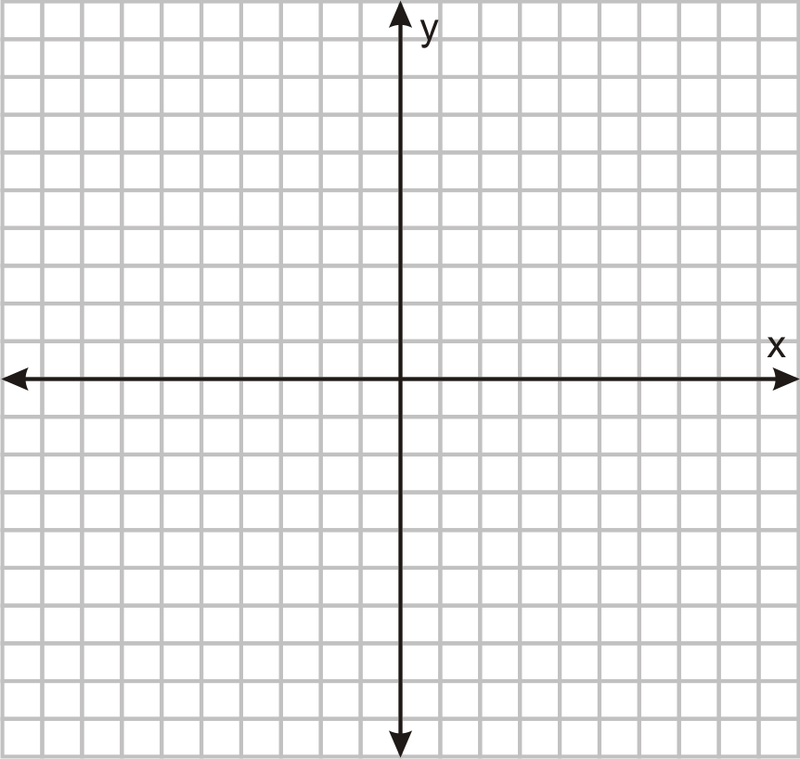
\includegraphics[width=1in]{../images/map}
        
\includegraphics[width=1in]{../images/cube}
    \end{minipage}
\end{frame}

\ifpre
\begin{frame}{The End}
  \centering \huge
  Thank You!
\end{frame}
\fi
\end{document}